
\documentclass[10pt,a4paper]{article}

\usepackage[T1]{fontenc}
\usepackage[utf8]{inputenc}
\usepackage[swedish]{babel}
\usepackage{comment}
\usepackage[round]{natbib}
\usepackage{amsmath}
\usepackage{amsfonts}
\usepackage{amssymb}
\usepackage{graphicx}
\usepackage{rotating}
\usepackage{multirow}
\usepackage{multicol}
\usepackage{float}
\usepackage{lscape}
\usepackage{longtable}
\usepackage{threeparttable}
\usepackage{authblk}
\usepackage{url}
\usepackage{booktabs}
\usepackage{subfigure}
\usepackage[margin=1.5in]{geometry}
\usepackage{placeins}         % Permets de vider le buffer de flottants avec \FloatBarrier
\usepackage{epstopdf}
\usepackage{pgfgantt}


\usepackage{color,framed}            % Utilisation des couleurs et de l'environnement shaded
\definecolor{shadecolor2}{rgb}{.92,.92,.92} % choix de la teinte de ``shaded''
\definecolor{shadecolor}{rgb}{.6,.95,.6} % choix de la teinte de ``shaded''
\usepackage[pagebackref=true,
            colorlinks=true,
            linkcolor=blue,
            anchorcolor=blue,
            citecolor=blue,
            filecolor=blue,
            menucolor=blue,
            urlcolor=blue,
            plainpages=true,
            pdfpagemode=UseThumbs,
            pdftitle={Titre},
            pdfauthor={ORDECSYS},
            pdfsubject={Sujet},
            pdfstartview=FitH]{hyperref} % Extensions PDF
\def\pdfBorderAttrs{/Border [0 0 0] } % Options PDF (No border around Links)
\renewcommand\Affilfont{\itshape\small}
\linespread{1.5}


\begin{document}

\title{Renewable Energy and Nuclear Phase out in Sweden}
%\title{Nuclear Phase out in Sweden}
\date{}
\author{}
\maketitle

\section{Summary}
Sweden has the ambition of showing the way to a sustainable society and needs to invest in economics research to better understand the impacts of ambitious energy policies. There is a great parliamentary divide on the perception of nuclear power, spanning from replacement of old reactors to a rapid phase out. A restriction in the supply of nuclear power will most likely have major economic consequences in a country like Sweden with a large element of power-intensive industries dependent on a stable and affordable supply of electricity. The research project we are proposing here intends to analyze the socio-economic costs and effects of restrictions on nuclear power capacity in combination with an expansion of renewable weather dependent power sources, in Swedish electricity production. With the type of CGE model we propose, it will be possible to analyze the effects of policy measures targeted at singular as well as groups of power sources in a system perspective. The tool will be an important contribution to the analysis ability of Swedish energy policy in general and policies targeting phase out of nuclear power in particular.
\section{Popular scientific description (in Swedish)}
Det råder parlamentarisk oenighet i frågan om kärnkraftens vara eller icke vara i den svenska energipolitiken. En begränsning i utbudet av kärnkraften kommer sannolikt att få ekonomiska konsekvenser i ett land som Sverige med ett stort inslag av elintensiv industri beroende av en stabil elförsörjning. Det forskningsprojektet vi föreslår avser att analysera samhällsekonomiska kosekvenser och spridningseffekter av restriktioner på svensk kärnkraftskapacitet i kombination med en utbyggnad av förnybar elproduktion. För att åstadkomma detta kommer vi konstruera en allmänjämnviktsmodell med fokus på energimarknaderna. Allmänjämviktsmodellers förmåga att beskriva ekonomiövergripande effekter utgör en viktig skillnad jämfört med andra så kallade partiella modeller. En allmänjämviktsmodell kan fånga upp de återverkningar som sker mellan olika sektorer vid förändringar av ekonomiska förutsättningar och inte bara den direkta påverkan i de berörda sektorerna. Jämfört med partiella modeller fångas de totala samhällsekonomiska konsekvenserna upp på ett mer fullständigt sätt i allmänjämviktsmodeller. Med den typ av allmänjämviktsmodell som vi föreslår, är det möjligt att analysera effekterna av politiska åtgärder riktade till såväl individuella som grupper av kraftkällor i ett systemperspektiv. Verktyget kommer att vara ett viktigt bidrag till förmågan att analysera den svenska energipolitiken i allmänhet och åtgärder som riktar sig utfasning av kärnkraften i synnerhet.
\section{Total project budget}
\section{Research programme (Appendix A)}
\subsection{Purpose and aims}
The research project we are proposing here intends to analyze the socio-economic costs and effects of any restrictions on the capacity of the nuclear power combined with an increased demand for balancing power, due to plans of expansion of renewable weather-dependent power sources. The goal is to analyze different scenarios under which the Swedish nuclear power system might develop over the next couple of decades. To this end, an existing CGE model is targeted for enhancement on detailed description of the Swedish energy sector. This type of model, called a hybrid model, is a combination of detailed micro data on the energy sector and more aggregated data usually used in computable general equilibrium (CGE) models. This hybrid model describes the energy sector in sufficient detail enabling analysis of changes in the economic conditions of different power sources for electricity generation. This type of CGE model is missing for the Swedish economy and would be a genuine contribution to the analysis of energy policy in general, but also a particularly well adapted tool for the project we are proposing here.

Energy issues are becoming increasingly important and related considerations increasingly complex. Surprisingly, energy economics is today a neglected field at Swedish universities, at least at the economics departments. CERE has launched a significant effort in this subject field. An important reason is the need for development of knowledge in CGE modeling in Sweden with focus on energy issues. Seeing the energy policy developments in a system perspective also seems increasingly important, especially in view of what has happened in the energy markets today.

Water for hydropower can be stored in ponds and production can efficiently adjust to the demand for electricity or variation of another generation which makes it very important in the Swedish energy system. It is especially important in an energy system that is including more renewable weather-dependent sources, such as solar and wind power. Hydropower also has a function as base load\footnote{The minimum amount of electric power delivered or required over a given period at a constant rate.} in the Swedish electricity mix due to its large share of the Swedish electricity production mix. Another important component in the Swedish electricity supply is nuclear power. Nuclear power function as provider base load power in Sweden and is not as important in terms of balancing fluctuating electricity demand, but represent a large share of total electricity generation in the base load section of the electricity maix. A reduction in the base load capacity by reducing or decommission the nuclear power while at the same time increasing weather-dependent sources will put a stress on hydropower in terms of both increased base load requirement and increased balancing demand at the same time. This will most certainly have impact on the scale as well as the stability of the Swedish electricity system.

There is some consensus among the leading parliamentary parties on electricity policies regarding securing hydropower, they welcome more renewable energy, and opportunities to work with energy efficiency. The great dividing line and the main conflict lies in the perception of nuclear power. The spectra lies between those who want a quick phase out, and those who are willing to replace existing reactors.

An important question in this political setting is to what degree the Swedish economic system will adapt to potential major changes in the electricity production system. A restriction in the supply of nuclear will most likely have major economic consequences in a country like Sweden with a large element of power-intensive industries dependent on stable supply of electricity. Furthermore, it is important to try to assess the spillover effects of such restrictions on the wider economy. This requires, in principle, detailed knowledge of every market in the country's economy and how these markets interact. A typical economic model to analyze this type of interaction between markets is the so-called general equilibrium model.

CERE has recently started a group (CGE Group) to specifically analyze the Swedish and European environmental and energy policies with the help of so -called general equilibrium modeling (CGE). CGE models' ability to describe the economy-wide effects is an important difference compared with different types of partial models. A CGE model can capture the repercussions that occur between different sectors and not only the direct impact in the sectors concerned. Compared with partial models captured the overall socio-economic impact on a more complete way in CGE models. The model we propose will be built upon a model constructed by Martin Hill for specific use in the Long-Term Survey 2008, but it became something of a workhorse for various investigations within the Treasury Department and has also been used for a number of studies of Swedish climate policy.

With the type of CGE model we propose, it will be possible to analyze the effects of policy measures targeted at individuals as well as groups of power sources in a system perspective. The tool will be an important contribution to the analysis ability of Swedish energy policy.

\begin{comment}
Question: Given a ambitious target for the share of renewable energy for Sweden (70 percent), how much nuclear power will fit in the system of electricity production? Answer: The excess electricity will be exported due to the low marginal cost of production of nuclear power. Follow up question: How and how much can we increase the cost of producing nuclear power in order to make it leave the market?

A nuclear phase out of Swedish nuclear power will be a process that evolve over time and should be modeled as such in order to capture the adaption of the Swedish economic system over time. Capital adjustment over time in dynamic CGE model bla,bla,bla...
Cost of disposal of nuclear waste

Time to time, requirement of imminent nuclear phase out emerge, most recently in a motion for the Swedish parliament (Motion 2013/14:N430) which states that nuclear power is redundant and that Sweden is equipped with means to supply all electricity demand from renewable sources. An other motion for the Swedish parliament (Motion 2013/14:N334) concludes that the Swedish nuclear power is heavily subsidized and urges substantial increases in both upper limits of liability cost of nuclear accidents (9000 percent increase) and mentions an increase of the cost per kilowatt producing set aside for funding nuclear waste storage at 350 percent.

Motif for renewable energy/electricity:
global warming - fossil fuel dependency (security of supply) - green jobs
In order to limit global warming to two degrees Celsius, reducing the EU's dependence on imports of fossil fuels and stimulate the growth of new green jobs is a sharp increase in the share of renewable energy in Europe absolutely necessary.


The Swedish nuclear power plants are old and according to current law it is possible to replace them.

Cap on hydropower:
feasible sources wind and biofuels

Assumptions on electricity demand

Motion 2013/14:N430
Kärnkraftsavveckling

Question 1:
Impact on hydropower as both base load and as a regulator of increased intermittent electricity requirement increase...

Motion 2013/14:N334
Avskaffa kärnkraftens subventioner

Question 2:
Ansvarsbelopp 11 GSEK vs 1000 GSEK
Capital adjustment over time in dynamic CGE model bla,bla,bla...

Question 3:
Cost of disposal of nuclear waste
I oktober 2011 föreslog SSM en höjning av den avgift kärnkraftsindustrin betalar till Kärnavfallsfonden från cirka 1 öre/kWh producerad kärnkraftsel till cirka 3 öre/kWh. Den 22 december 2011 beslutade regeringen att endast höja avgiften till 2,2 öre/kWh. Under 2013 meddelade Kärnavfallsfonden att det ändå saknas över 30 miljarder kronor för att de avsatta pengarna ska räcka till slutförvaret av det svenska kärnavfallet. Enligt en uträkning som Sveriges Radio Vetenskapsradion låtit göra skulle avgiften behöva femfaldigas till runt 10 öre/kWh för att täcka upp underskottet i Kärnavfallsfonden.
\end{comment}


\subsection{Survey of the field}
Globally, nuclear energy contribute around 14\% for the world electricity generation \citep{OECD2012}. Many countries in Europe depend on nuclear energy for the electricity generation with 75\% in France , 54\% in Slovak Republic , 51\% in Belgium\footnote{http://www.iaea.org/PRIS/WorldStatistics/NuclearShareofElectricityGeneration.aspx}. About 40\% of total Swedish electricity generation in 2011 was produced from nuclear energy \citep{SEA2012}. However, the future of nuclear power is considerably uncertain in different countries due to economic, technological, environmental and political factors \citep{Joskow2012}. On one hand, nuclear power continues to generate enthusiasm based on its potential to reduce greenhouse gas emissions and comparatively cheaper to renewable energy \citep{Davis2012, Renssen2013}. On the other hand, there is growing opposition against nuclear power regarding its safety measures, handling and storage of spent fuel, proliferation of nuclear weapons. After the Fukushima nuclear disaster, Germany and Switzerland have decided to phase out the nuclear power completely from their energy portfolio by  2022 and 2034 respectively. The position taken by Germany and Switzerland points to the potential tension between a need for climate mitigation and a desire for a society free from nuclear power \citep{Glomsrod2013}. It is quite likely that Sweden faces similar challenges in coming future whether to phase out nuclear power or not with ambitious emission targets for 2030. Without well defined capacity replacement plan, the countries could face a severe shortage of electricity supply and significant cost to the society. In this current context, it is important to understand what could be an economic implication of nuclear phase out for Sweden. How this will impact the electricity market and emissions in Sweden?

Several studies have shown the potential economic consequences of nuclear phase-out \citep{Bohringer2002, Nestle2012, Bretschger2012, Duscha0, Glomsrod2013, Kunsch2014}. Temporary halt or phasing out of nuclear reactors would entail more electricity generation from the other sources to meet a given demand. Subject to the constraint on capacity, the substitution follows a merit order of marginal costs of generating electricity from different sources \citep{Glomsrod2013}. The study by \cite{Bretschger2012} showed the nuclear phase-out can be achieved at relatively low costs even when the expansion capacities of other technologies are limited. This is achieved by innovation and structural shift to less energy dependent economy. Similarly, there are several studies done in the case of Germany \citep{Bohringer2002, Nestle2012}. The study by \cite{Bohringer2002} found that alternative regulation leading to same phase-out date can have distribution of of phase-out costs across companies changes considerably for the various regulation schemes, revealing an important equity dimension of phase-out policies. The evidence is presented suggesting that extending nuclear plant life spans or the commissioning of new reactors in other countries is unlikely to curb domestic electricity prices \citep{Nestle2012}. The study by \cite{Kunsch2014} found that a too early nuclear phase out will indeed benefit to fossil fuel, creating unwanted drawbacks regarding safety of supply, dependency on foreign suppliers, price volatility, and increased use of non-renewable and CO2 emitting fossil fuels.

There are only few study done this in Swedish context. The study by \citep{Bergman1981} used a general equilibrium model and showed that given that the product and factor markets to function smoothly and to full utilize the economy's resources, Sweden can accommodate quite significant changes in electricity supply conditions without major changes in main economic indicators. However, adjustment cost (reallocation of labor force, transportation cost, capital losses etc.) which are neglected in the model could give quite different results. While, the study by \cite{ Andersson1997} used partial equilibrium model and showed that phasing out nuclear power while restricting future CO2 emissions to the 1990 level implies a significant increase in electricity prices and a substantial loss in welfare. Furthermore, it is important to study the current ongoing debate on nuclear phase-out in the present Swedish energy and economic context with energy and climate policy objectives.

\begin{comment}
Nuclear safety and waste disposal.: Number of people surrounding nuclear power plant at 30 km radius.
Current political situation regarding nuclear phase out in Sweden: What current government says and what its opposition parties says
To represent the government plan,
To represent the opposition parties plan,
Potential role of hydropower, renewable and carbon capture and sequestration.
Current energy status of Sweden.
Considering the nuclear power to be phase out, and the possibility of substituting it by relatively in expensive technique of fossil fuel power is excluded due to CO2 commitment and hydropower development is restricted due to its capacity, then the price and supply of electricity will most certainly be affected.

To expand hydroelectric power or to revert to importing oil and gas to substitute for nuclear energy are hardly options for an environmentally conscious state like Sweden. Moreover, replacing nuclear power with renewable energy sources is not currently a realistic option.

The purpose of this research is to examine the effects of different policy scenarios with respect to Swedish energy policy, specifically issues concerning a nuclear phase-out and restrictions on CO2 emissions.

\end{comment}



\subsection{Project description}
%Summarise the project. Describe theories, methods, timetable, implementation and project organisation.
As mentioned in the section 1, a computable general equilibrium model will be used for the purpose of our research. A CGE model is theoretically consistent with microeconomic foundations. In such a model, each sector and consumer optimizes their production and consumption decision at different stages of production and utility tree within their resource and budgetary constraints, respectively. These models also ensure the balance of income and expenditure of the economic agents, market clearing conditions (supply is equal to demand) and zero profit conditions (sum of inputs is equal to output) for each sector (commodity). Moreover, it can simulate not just parts of the economy that are of interest but also of the entire economy. Hence, a CGE model becomes appropriate in this research when a nuclear phase out policy not only affects the electricity sector, but also will have economy-wide effects. These models are also useful for analyzing changes in sectoral output, prices, endowments and trade as well as changes in national efficiency (welfare) consequent to policy changes.

A feature of the Swedish electricity production system is that major parts as hydropower and nuclear power are subject to caps on the production capabilities. The growth of hydropower is restricted to limited increases in the efficiencies of their turbines and the restricted capacity of nuclear power is the target for the analysis. These types of capacity constraints are well suited to be modeled under the mixed complementarity framework \citep{raey} which we will use for our proposed project.

\begin{comment}
\textbf{Modeling electricity sector}
Disaggregated electricity sector
- Coal, Gas, Oil, Nuclear, Hydro, Wind
- to incorporate natural resource constraints on hydro and wind, the expansions of wind and hydro power are bounded by the levels of hydro and wind resource factors, respectively.

\textbf{Scenarios}
- Scenario 1: Phase out of existing nuclear power (without expansion of hydro power plant)
- Scenario 2: Phase out of existing nuclear power plant (with expansion of hydro power plant)
- Scenario 3: Phase out of existing nuclear power plant (without expansion of hydro power plant) and CO2 commitment
- Scenario 4: Phase out of existing nuclear power plant (with expansion of hydro power plant) and CO2 commitment

\end{comment}


% timetable, implementation and project organisation



% Implementation
% Data
An initial step for the project is to compile a so-called social accounting matrix (SAM), for Sweden, with specific focus on the energy markets. This work involves the collection of data from different sources and processing of these data so that they can consistently describe the Swedish economy in equilibrium and that the data are of sufficient detail to adequately analyze policies targeting the electricity system. This SAM will feed the model with new and complementary data.
% Model enhancement and scenarios
The existing base model will have to be modified in order to incorporate the new detailed data for the Swedish energy system and calibrated to current economic situation in order to establish a benchmark to compare with relevant policy simulations. Scenarios of different potential policy decisions will be created, and the model will need further modification in order to accommodate simulations of these scenarios.
% Paper writing (how many)
The research group will in cooperation write papers for peer-reviewed scientific publication and results will be presented at international meetings, workshops and conferences. We will make a special effort to put our results into popular science forums to facilitate the spread of knowledge outside the academic arena.
% Timetable
The most time consuming part of the project will be the compilation of the SAM and we estimate that this will be accomplished during the first year. Model modifications, creation of relevant scenarios for simulations, and paper writing will take place during both of the years of the project.
% Project organisation
The research group operates within the Centre for Environmental and Natural Resource Economics, CERE. CERE is an interdisciplinary research center that unites Umeå University (UmU) and the Swedish University of Agricultural Sciences (SLU). Many prominent researchers are cooperating with CERE comprising an exclusive and important international network. A general aim of CERE is to provide high class research on topics pertaining to energy systems. Of special interest are the effects of climate and energy policy on energy use, which the proposed project aims to study. A well-established and experienced group of researchers can without doubt compose a notable contribution in analyzing and assessing relevant energy issues.\\*
The research group consists of:\\*
\textbf{Dr. Örjan Furtenback} CERE Natinal institute for economic research, bla, bla ...\\*
\textbf{Dr. Joshi Santosh Ram} a PhD from NUI Galway, Ireland, and a Master from Wageningen University. He has previously worked as a modeler at the Economics and Environmental Laboratory in Switzerland. His research at CERE will in general be focused on computable general equilibrium modeling, and especially on integrating a detailed description of the energy sector into a Swedish model.\\*
\textbf{Professor Chris Böhringer}; a world leading authority on Computable General Equilibrium (CGE modeling), research associate at ZEW in combination with his chair at the Department of Economic Policy at the University of Oldenburg, Germany. Beside collaborating in this project Professor Böhringer has been connected to CERE and Umeå and will be an important part of the CERE strategy to develop CGE modeling – particularly within the framework of our general work on energy issues.\\*
\textbf{Dr. Martin Hill}, employee at the Ministry of Finance and Adjunct Professor to SLU and CERE, is one of Sweden's most skilled CGE specialists and will function as an collaborating member of the group.\\*
\textbf{Dr. Badri Narayanan}, researcher at the Center for Global Trade Analysis, Department of Agricultural Economics, Purdue University, USA. Dr. Narayanan holds an extensive knowledge in data issues regarding CGE modeling and will be an tremendous asset in the labor intense work of constructing the SAM.\\\\
\begin{comment}
The efficient implementation of the project requires proper organisation. Two researcher engaged in the project will have regular meeting to ensure that purpose and aim of the project are going in right direction with the supervision of the team leader. Meeting with the international expert who are experts on this field will guarantee that the research work is of international standard with scientific quality and policy relevance.
\end{comment}

\vspace{1cm}

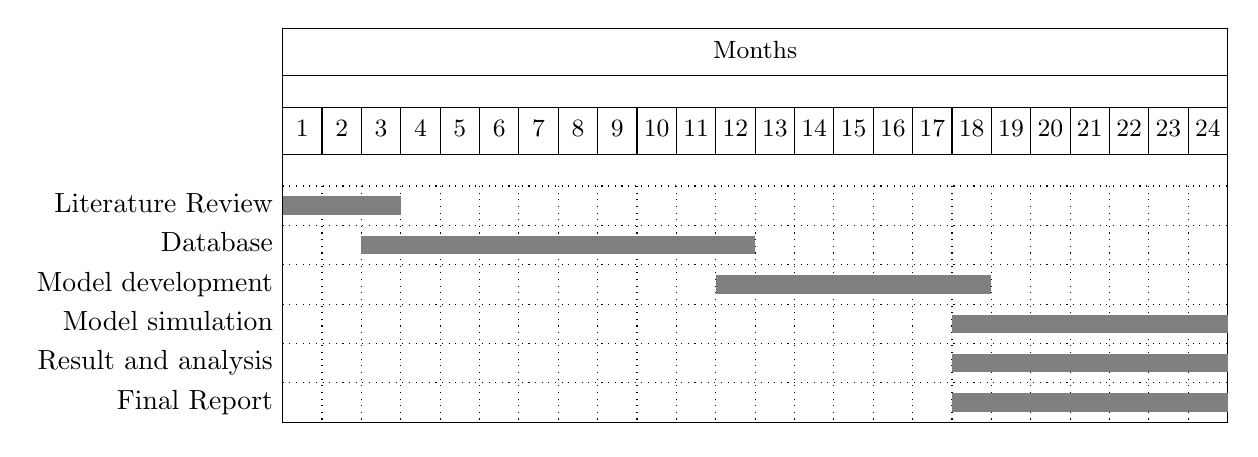
\begin{tikzpicture}[y=0.5cm]  
\begin{ganttchart}[
hgrid=true,
vgrid= true,
y unit chart=0.5cm,
bar/.style={fill=gray}
]{1}{24}
\gantttitle{Months}{24} \\
\gantttitlelist{1,...,24}{1} \\
\ganttbar{Literature Review}{1}{3} \\
\ganttbar{Database}{3}{12} \\
\ganttbar{Model development}{12}{18} \\
\ganttbar{Model simulation}{18}{24} \\
\ganttbar{Result and analysis}{18}{24} \\
\ganttbar{Final Report}{18}{24}
\end{ganttchart}
\end{tikzpicture}

%http://ctan.mirrorcatalogs.com/graphics/pgf/contrib/pgfgantt/pgfgantt.pdf

\subsection{Significance}
Having the ambitious emission targets and the safety and disposal issue relevant for nuclear power, there is an urgent question whether Sweden should phase out, early phase out and replace its ageing nuclear power, or not. If Sweden decide on these possible options, it is important to carry out an analysis of its impact on Swedish economy and energy system. There are only a few attempts in the past to investigate the socio-economic consequence of nuclear phase out in Sweden. Since these studies, economic and energy systems in Sweden has evolved and changed considerably and hence this project seeks to advance in this research area within the Swedish context. This will be achieved by using a recent database, incorporating detailed energy and electricity system, and developing relevant scenarios that are required to model the implications of a nuclear phase out. This research will add to the academic discourse on the issue of nuclear phase out and ultimately answer pertinent policy questions to give guidance to decision and policy making.

\subsection{Preliminary results}
Researchers of this project have used CGE model extensively in their research area. The Global Trade Analysis Project (GTAP), a multi-regional, multi-sectoral static general equilibrium model, was used to analyse the implication of WTO trade policies. To examine and analyse complex multi-sectoral and multilateral trade negotiations as are contained in the WTO trade policies ,a global economic model such as GTAP is required. Similarly, GEMINI-E3 (General Equilibrium Model of International-National Interactions between Economy, energy and Environment), a recursive dynamic CGE model, is used to do macroeconomic analyse of the impacts and adaptation to climate change. This model was linked with other systems of models (climate, energy and agriculture) to get wider perspective and implications of climate change. This research was part of Framework Programme 7 project ERMITAGE (Enhancing Robustness and Model Integration for The Assessment of Global Environmental Change).
In the Swedish setting the CGE-model EMEC (Environmental Medium term Economic model) of the National institute for economic research in Sweden was used to account for forest sequestration in the analysis of the Swedish vision on carbon dioxide emissions for 2050 as well as the 2030 goal for fossil fuel independence.
\subsection{National and International collaboration}
Christopher Böhringer\\*
Badri Narayanan Gopalakrishnan\\*
Martin Hill\\*
% Add to traveling expences

\section{CV (Appendix B)}
\section{Publication list (Appendix C)}
\section{Budget and research resources (Appendix N)}
The budget for the project consists mainly of salaries to researchers. A small part is funding
for collaboration, travel and data. In total we seek X TSEK which is distributed as follows:\\*
Örjan Furtenback, salary: X TSEK\\*
Researcher.\\*
Joshi Santosh Ram, salary: X TSEK\\*
Researcher.\\*
Collaboration, travel and data: X TSEK\\*
This is mainly aimed at traveling expenses for collaborators Chris Böhringer, Martin Hill and Badri Narayanan Gopalakrishnan. As guest Professor at CERE, Professor Böhringer will partly be funded internally
by CERE during the project.\\*
For more information about the research group and collaboration see project description.
\section{Signatures (Appendix S)}



\pagebreak
\addcontentsline{toc}{chapter}{Bibliography}
\bibliography{RefAbstracts}
\bibliographystyle{plainnat}

\end{document}
